\documentclass[12pt]{article}
\usepackage[margin=1in]{geometry}
\usepackage[utf8]{inputenc}
\usepackage{amsfonts}
\usepackage{amsmath}
\usepackage{amsthm}
\usepackage{tikz-cd}
\usepackage{tipa}
\usepackage{graphicx}
\usepackage{float}
\usepackage{hyperref}
\usepackage[numbers]{natbib}

\bibliographystyle{IEEEtran} % shows URL
\setcitestyle{square,numbers}

%%% Common categories
\newcommand{\tp}{\;\mathrm{type}}
\newcommand{\Hom}{\mathrm{Hom}}
\newcommand{\G}{\Gamma}
\newcommand{\pit}[1]{\prod_{(#1)}} % pi-type
\newcommand{\pitxa}{\pit{x:A}}
\newcommand{\sit}[1]{\sum_{(#1)}} % sigma-type
\newcommand{\ent}{\vdash}
\newcommand{\adj}{\dashv}
\newcommand{\refl}{\ensuremath{\textsf{refl}}}
\newcommand{\ap}{\ensuremath{\textsf{ap}}}
\newcommand{\ind}{\ensuremath{\textsf{ind}}}
\newcommand{\lift}{\ensuremath{\textsf{lift}}}
\newcommand{\inv}{\ensuremath{\textsf{inv}}}
\newcommand{\concat}{\ensuremath{\textsf{concat}}}
\newcommand{\transport}{\ensuremath{\textsf{transport}}}
\renewcommand{\sec}{\ensuremath{\textsf{sec}}}
\newcommand{\retr}{\ensuremath{\textsf{retr}}}
\newcommand{\total}{\ensuremath{\textsf{total}}}
\newcommand{\isequiv}{\ensuremath{\textsf{is\_equiv}}}
\newcommand{\fib}{\ensuremath{\textsf{fib}}}
\newcommand{\id}{\ensuremath{\text{id}}}
\newcommand{\judgeq}{\ensuremath{:\equiv}}
\newcommand{\reflfx}{\ensuremath{\refl_{f(x)}}}

\newcommand{\rr}{\ensuremath{\mathbb{R}}}
\newcommand{\rrn}{\ensuremath{\mathbb{R}^n}}
\newcommand{\rrm}{\ensuremath{\mathbb{R}^m}}
\newcommand{\rrx}{\ensuremath{\mathbb{R}[x]/x^2}}
\newcommand{\rry}{\ensuremath{\mathbb{R}[y]/y^2}}
\newcommand{\cc}{\ensuremath{\mathbb{C}}}
\newcommand{\nn}{\ensuremath{\mathbb{N}}}
\newcommand{\dd}{\ensuremath{\mathbb{D}}}
\newcommand{\vv}{\ensuremath{\mathbb{V}}}
\newcommand{\cinfty}{\ensuremath{C^{\infty}}}
\newcommand{\smfd}{\textsf{SmoothMfd}}
\newcommand{\calg}{\textsf{CAlg}_{\rr}}
\newcommand{\cart}{\textsf{CartSp}}
\newcommand{\formalcart}{\textsf{FormalCartSp}}
\newcommand{\formalsmoothset}{\textsf{FormalSmoothSet}}
\newcommand{\smoothset}{\textsf{SmoothSet}}
\newcommand{\setcat}{\textsf{Set}}
\newcommand{\psh}[1]{\textsf{Psh}(#1)}
\newcommand{\sh}[1]{\textsf{Sh}(#1)}
\newcommand{\pshcart}{\psh{\cart}}
\newcommand{\rmodal}{\Re}
\newcommand{\imodal}{\Im}
\newcommand{\shape}{\ensuremath{\text{\textesh}}}
\newcommand{\op}[1]{#1^{\textsf{op}}}
\newcommand{\pt}{\mathrm{pt}}
\newcommand{\Aut}{\mathrm{Aut}}
\newcommand{\BAut}{\mathrm{BAut}}
\newcommand{\im}{\mathrm{im}}
\newcommand{\Fin}{\mathrm{Fin}}
\newcommand{\Type}{\mathrm{Type}}
\newcommand{\pinv}{p^{-1}}
\newcommand{\aut}{\mathrm{Aut}}

\newcommand{\bg}{\ensuremath{\textbf{B}G}}
\newcommand{\bgconn}{\ensuremath{\textbf{B}G_{\textsf{conn}}}}
\newcommand{\bgdiff}{\ensuremath{\textbf{B}G_{\textsf{diff}}}}

\newcommand{\gc}[1]{\marginpar{\bf $\leftarrow$ {#1}}}
\newcommand{\comment}[1]{}
%\newcommand{\gc}[1]{}

\newtheorem{mydef}{Definition}
\newtheorem{mythm}{Theorem}
\newtheorem{mylemma}{Lemma}
\newtheorem{myprop}{Proposition}
\newtheorem{myclaim}{Claim}

\title{Connections on principal bundles}
\author{Greg Langmead}
\begin{document}
\maketitle
\begin{abstract}
These notes are intended as a didactic presentation of connections on principal bundles. I assume the reader knows some toplogy, such as the definition of compactness, and the preliminaries of differential geometry such as the definition of smooth manifolds and Lie groups. The goal is to define connections and Chern-Weil theory and then go through the paper by Freed and Hopkins \cite{freed2013chernweil} and finally sketch how we can import all of these ideas into type theory.
\end{abstract}
\tableofcontents
\section{Introduction}
If you are interested in these notes but worry about whether you have the prerequisites, let me offer two of my favorite resources. First is the book by John Baez and Javier Muniain \cite{baez1994gauge} which is a compact and beautiful introduction to manifolds, connections, and the physics that uses these concepts. I'm still not sure why fate did not put this book in front of me in graduate school, when I was voraciously hunting on an almost daily basis for books just like it.

If, like me, you do even better with recorded lectures, I strongly recommend the playlist of lectures by Frederic Schuller \cite{schullerYoutube2015}. His course is efficient but very precise, and he is a great teacher who offers helpful intuition along the way. The scope is similar to the book by Baez and Muniain: he begins with topology and manifolds, defines connections and curvature, and then gets into physics.

\section{Lecture 1 outline}
Start with picture of S2 embedded in R3 and draw intuitive transport pictures.

The central intuition is below, the splitting thing.

Formulas: change-of-chart transformation for connection.

Principal bundle version: equivariance.

Composition with maps to/from Lie algebra.

Covariant derivative.

\section{Motivation and Plan}
Why study connections? I have two answers. The first is to tell you a little about the Chern-Weil theory of characteristic classes. Just as we strive to construct topological invariants of manifolds that are functorial, we may strive to construct topological invariants of \emph{bundles} over manifolds. The theory of characteristic classes provides cohomology classes on the base that depend only on the isomorphism classes of the bundle. This is global stuff -- dependent on the way the maniofold twists or has holes, and the way the bundle twists over that space. But Chern-Weil theory gives us a way to compute characteristic classes making use of a connection (in fact, just the curvature of the connection) which is a local construction! This theory generalizes the Gauss-Bonnet theorem which states that if $M$ is a compact 2-dimensional manifold without boundary and with Euler characteristic $\chi(M)$, then we have $$\chi(M) = \frac{1}{2\pi}\int_M K dA$$ where $K:M\to\rr$ is the \emph{scalar curvature}, which is where the connections come in, and $dA$ is a measure on the manifold compatible with the connection.

For example, the standard 2-sphere embedded in $\rr^2$ has constant curvature and so we'll get some positive number when we integrate that everywhere, which is consistent with the euler characteristic being positive. Meanwhile a torus embedded donut-style in $\rr^3$ has regions of positive curvature (along the outside ring where you bite), and regions of negative curvature (along the inside ring where it's saddle-shaped) and it will all cancel out to zero. Performing the integral passes from local to global, and curvature is the thing to integrate to compute a topological invariant. That's Chern-Weil theory in a nutshell.

The second motivation is from physics. The force-carrying fields such as photons for electromagnetism, or gluons for the strong force, are as usual not point particles, but fields. They are not plain old functions though, like you meet in a first course on quantum mechanics where you consider $\psi:\rr^4\to \rr$. Rather, these quantum fields are connections. In EM theory the connection's 1950s name was the "electric potential", and the curvature, which is the differential of the connection, contains all six components of the electric and magnetic fields.

The beautiful thing that happens next is to look at the space of all connections, or the space of all bundles plus a connection. This is known as \emph{gauge theory}, and leads in turn to a quantum version of Chern-Weil theory where invariants can be defined by integrating formulas over this whole space. We'll be interested eventually in figuring out how to define this space as a groupoid or other higher type. That's the entirety of the plan!

\section{Fiber bundles}
We start in the category of smooth manifolds and smooth maps. A fiber bundle consists of a surjective map $p:E\to M$ and a space $F$ such that for every $x\in M$ there is a neighborhood $U$ of $x$ diffeomorphic to the product $U\times F$ in a way that respects the fibers.

\[\begin{tikzcd}
	{p^{-1}U} && {U\times F} \\
	& U
	\arrow["p", from=1-1, to=2-2]
	\arrow["\phi", from=1-1, to=1-3]
	\arrow["{\mathrm{pr}_1}"', from=1-3, to=2-2]
\end{tikzcd}\]
So $E$ is a type family over $M$, plus this local product condition. We can also write $E|U$ for $p^{-1}U$. The maps $\phi$ go out of the bundle, into the product. The overlaps have a group structure. Fix a cover of $M$ consisting of sets $U_\alpha$ and product maps $\phi_\alpha:p^{-1}U_\alpha \to U_\alpha\times F$. Then $\phi_\beta\circ\phi_\alpha^{-1}: U_\alpha\times F\to U_\beta\times F$, fixing the first factor, and so give a map $\phi_{\alpha\beta}(x): F\to F$ for each $x\in U_\alpha\cap U_\beta = U_{\alpha\beta}$, hence $\phi_{\alpha\beta}:U_{\alpha\beta}\to \mathrm{Diffeo}(F)$. 

A vector bundle is where $F$ is a vector space and the overlap functions land in $GL(F)\subset\mathrm{Diffeo}(F)$. A principal bundle is where $F$ is a Lie group and the overlap functions land in $\aut(G)\subset \mathrm{Diffeo}(F)$, plus another condition we'll get to shortly.

Brief aside on how I talk about vector bundles. Given two bundles over the same base, say $p:E\to M$ and $q:F\to M$, we can form $r:E\otimes F\to M$ by taking the tensor product fiberwise. This gives vector bundles with a fixed base a monoidal structure. When we talk about sections of such tensor products, we sometimes use language like ``a section of $E$ with values in $F$." In the special case where $E$ is $T^*M$, the dual of the tangent bundle, such a section is called ``a 1-form with values in $F$."

Defining a connection requires looking at tangent bundles. It might be helpful to think of the tangent bundle as an endofunctor in the category of smooth manifolds, where on objects it forms the tangent bundle of the manifold, which is a new manifold, and on maps it takes the derivative of the map. The projection maps of the tangent bundles down to their bases is a functor in the other direction. Thus we have $$Tp:TE\to TM.$$ \gc{expand a bit}

The map $Tp$ has as kernel the vertical-pointing tangent vectors, i.e. those that point along the fiber, a $\dim F$-dimensional subspace of $TE$ at each point. This kernel is a sub-bundle of $TE$ we call $VE$.

There's enough structure here to form the following short exact sequence, which is a central object of our study: $$0\to VE\to TE \to p^* TM\to 0.$$
\comment{https://mathoverflow.net/questions/245525/geometric-interpretation-of-horizontal-and-vertical-lift-of-vector-field/245576#245576}
\comment{Atiyah Sequences: Biswas paper and https://mathoverflow.net/questions/330797/atiyah-sequence-and-connections-on-a-principal-bundle}

A connection is a splitting of this exact sequence that varies smoothly. We can formulate that three ways:

\begin{enumerate}
\item A connection is a choice of complementary horizontal subspace of $TE$ at every point, i.e. a bundle $HE$ such that $TE=VE\oplus HE$. The horizontal subspace is isomorphic to $p^* TM$ by dimension-counting.

\item A connection is a projection $TE\to VE$. The kernel of this operator is the horizontal subspace. This operator is called a 1-form because it takes as input tangent vectors. We usually denote a connection 1-form with $\omega\in\Omega^1(E, VE)$.

\item A connection lifts some of the structure of $TM$ up to $TE$. Given a tangent vector $v_x$ in $T_x M$ and a point $e$ over $x$, we get a point in $p^* TM$. A splitting is then a map into $TE$, which embeds $p^* TM$ as a horizontal subspace of $TE$.
\end{enumerate}

Example on trivial bundle.

Prove existence of connections on any bundle.

Special case: $TM$.

Background on distributions.

Let's denote the lift by $L$, so $L_x v_x\in H_e E$ (and $pe=x$). If we have two vector fields $X$ and $Y$ on $M$ then we can lift them both. Once we lift them both we can do something interesting: we can form $[LX, LY]$ upstairs, and see if it has any vertical component, i.e. we can form $\omega[LX, LY]$. What if this is always zero? What if the bracket upstairs of two horizontal vector fields are always themselves horizontal? Then the sub-bundle $HE$ is what we call "integrable", and there exists a \emph{foliation} of $E$, which is a structure of local slices compatible with $HE$. This is called a \emph{flat} connection, and in this case we could run with the foliation and drop the use of tangent bundles.

A flat connection on $E$ is a foliation by $\dim M$-dimensional submanifolds.

Imagine now lifting a whole loop in $M$, but let's say it's contractible. If the connection is flat, then the lift is also a loop, because the whole loop lives in one leaf the foliation and so returns to its base point. In a general connection the loop may return to another point in the fiber above the base point in $M$. This gap is called \emph{holonomy}. 

\section{Principal bundles}
A principal bundle is a fiber bundle whose fiber is a Lie group $G$ and where there is a transitive and free right-action of $G$ on $E$ so that $M = E/G$. So each fiber is diffeomorphic to $G$ but in an affine sort of way without identity point. The canonical example of this is to take a vector bundle and form its bundle of frames, i.e. bases. The collection of bases of a vector space $V$ is such an affine copy of $GL(V)$. Fixing one basis $b$ then gives an identification with $GL(V)$ by mapping a frame $f$ to the transformation that takes $b$ to $f$.

At the level of descent data, where overlaps of neighborhoods of $M$ are mapped into a group, there is no difference between a principal bundle and a bundle of spaces on which the group is acting. Given an action of the group $a:G\times F\to F$ and a principal fiber bundle $P$, the fiber bundle with fiber $F$ that uses the descent data plus the action $a$ is called an \emph{associated bundle}.

A \emph{gauge transformation} is a $G$-equivariant diffeomorphism $f:P\to P$ covering the identity, so that $p\circ f = p$ and $f(u\cdot g) = f(u)\cdot g$. It's a group action on each fiber, but varying smoothly from fiber to fiber. In physics, observables are invariant under such transformations, just like they are invariant under Lorentz transformations.

A \emph{principal connection} on a principal bundle is a connection in the general sense of fiber bundles, plus the extra condition that the connection be $G$-equivariant. 

The vertical bundle is trivial, and in fact we have that $VE\cong E\times\mathfrak{g}$ by simply differentiating the $G$-action on $E$. Specifically, given $X\in \mathfrak{g}$, choose a curve in $G$ whose derivative at the identity is $X$, then take a point $u\in E$ and act on it with the curve, and take the derivative at the identity. This will be some vertical vector which we associate bijectively with $X$. This is handy and lets us talk about what's going on inside $TP$ by using the fact that the vertical part is made of $\mathfrak{g}$.



\section{Connections}
Vertical bundle. Connection as horizontal bundle. adP. Sequence being split, local version and integrated version.

Vertical bundle: Given $p:P\to B$, consider $TP$ and $p_*:TP\to TM$. Consider the kernel of $p_*$, which are all the vertically-pointing vectors. We define $T_F P = \ker p_*$. To define an appropriate complementary subspace to play the role of horizontal tangent vectors is to define a connection! 

Imagine we had such a decomposition $TP=T_FP \oplus T_HP$. Then imagine we have a tangent vector in the base to some point $x$ and some point $e$ in the fiber over $x$. Then we can uniquely lift that tangent vector to a horizontal tangent vector at $e$!. Next imagine we have a whole curve in the base $c:[0,1]\to B$ and a point $e$ in the fiber over $c$. We can lift all the tangent vectors and integrate them in $P$ to get a horizontal path??

Now let's fully define the horizontal sub-bundle.

Pullback of connections.
\section{Holonomy and HoTT}

\section{Towards connections}
To have connections we need both $TM$ and $TTM$. Eventually we need to define vector bundles $E$ as a slice category, and then we'll need $TE$. But in the case of $TTM$ how can we get there with an idempotent modality?

I think the key is to introduce a variable into the modal operator: $\imodal_x, \imodal_y$. At the algebra level these will come from $$\cinfty(\rrn)\otimes\rrx\otimes\rry = \cinfty(\rrn)\otimes\rr[x, y]/(x^2, y^2)$$. Each modal operator is idempotent. Adding the $x$ variable again doesn't provide more fuzziness, or more tangency, or more directions to differentiate in. But adding $y$ does.

It's crucial that the differentiation these variables are doing will commute with each other, so that it doesn't matter which one was tensored outermost.

Having the $x$ lets you differentiate everything, and adding $y$ lets you differentiate everything including the $x$ (i.e. there are now terms in $xy$).

If $\rrx$ leads to an interpretation of $\imodal_x$ then we can indeed have two of them.

I also want to add a functor $T$ with $TA=A[x]/x^2$ which I hope is equal to $A\otimes_{\rr}\rrx$. Perhaps the unit of this is the zero section. Then we would have two functors, $I$ and $T$, and the units are $p$ and $i$. We'll need better names. $T$ and $I$ are inverses on the nose. The Kan extensions will convert between sets of probes that can see the tangent space and those that cannot.

When there are two modalities, the Kan extensions will move between sets of probes that can see 0, 1 or 2 iterated copies of the tangent space.

There is always a map $TTM\to T_2 M=TM\times_M TM$, where the right hand side is the pullback of $TM$ by $p$, i.e. each fiber over $M$ is two copies of the tangent bundle.\gc{what about Lang's claim that $T_2 M$ is only a fiber bundle not a vector bundle?}

A connection is a section of this map, so $L:T_2 M\to TTM$. Given two tangent vectors you can lift that pair up to a vector in $TTM$, in fact a horizontal one. The image of the connection map is the horizontal sub-bundle of $TTM$. The kernel of the bundle projection is the vertical sub-bundle.

What types will we have? Apparently we'll have ones that "are $T$ of something" and ones that are not. If you are $T$ of something then you can be probed by nilpotents, and you are not coreduced. Else you are coreduced. To be $T$ of something you must be differentiable everywhere. Perhaps this is why $\sum_{a:A}B(a)$ is coreduced whenever $A$ is.

Infinitesimal closeness is preserved by morphisms. Equivalently, morphisms are bundle morphisms, they preserve the fibers. Is it also equivalent to stipulate that at the algebra level the morphisms hold $x$ fixed?

\section{Towards Chern-Weil, without coreduction}
\bgconn\ is: a non-concrete simplicial presheaf, and also a groupoid version of connections mod gague. The objects are connections and the morphisms are gauge transformations. In my thesis days, connections and connections mod gauge were talked about as analogous to $EG$ and $BG$ but with connections. This was only approximately true because some gauge transformations had fixed points and so it wasn't a principal bundle because the action wasn't free. All of this will fit more nicely into this framework I dare say.

There is a map $\bgconn\to\bg$. The bundles that these classify are trivial, not sure yet how to remedy that so that it can cover the frame bundle and other bundles that we need for the full Chern-Weil.

Urs and Baez-Huerta describe a theory of higher parallel transport. This is where contact is made directly with classical calculations and curvature.

In Baez-Huerta An Invitation to Higher Gauge Theory we find an elementary explanation about how a 2-connection on a (trivial?) 2-principal bundle associated with a 2-group is a connection plus its curvature. The intuition is simply that the holonomy functor acts on both paths and on squares that fill in the paths -- just like curvature. For everything to hang together 2-categorically the curvature appears exactly: $dA + A\wedge A$.

The technology of 2-connections was invented to support string theory. But if a flat 2-connection contains in it a regular 1-connection that might be curved, then it can also serve to put standard gauge theory in a form that is accessible to modal hott with shape modality, and hence to formalization.

Urs says that the flatness of one of the terms of a 2-connection is the Bianchi identity.

Do we package transport with a functor $\mathsf{tra}:\shape X\to \bg$?

Urs sez: A connection $\nabla$ is flat precisely if it factors through the inclusion $\flat \bg \to \bgconn$.

$\bgconn(X)$ restricts to the manifold $X$.

$$\left[ \op{\cart}, \mathsf{Grpd} \right](\textbf{P}_1(X), \bg) \simeq \bgconn(X)$$
$$\left[ \op{\cart}, 2\mathsf{Grpd} \right](\textstyle\int_2(X), \bg) \simeq \flat\bg(X)$$

Besides the 1 vs 2, we have $\textbf{P}$ vs $\shape$, which is the passage from paths to homotopy classes of paths, hence from connections to flat connections.

Focusing on homotopy classes of paths and higher paths focuses on flat connections and higher connections.

``For $G$ a Lie group, its inner-automorphism 2-group $\mathrm{INN}(G)$ is as a groupoid the universal $G$-bundle $EG$, but regarded as a 2-group with the group structure coming from the crossed module $G\to G$.''

\section{Freed-Hopkins: from connections to groupoids}
In Freed-Hopkins \cite{freed2013chernweil} they take a similar pov and construct a universal $G$-connection on a $G$-bundle $E_{\nabla}X\to B_{\nabla}X$ of which any given principal bundle \emph{with connection} is a pullback.

We want to construct invariants of $G$-principal bundles on a fixed base manifold $M$. Chern-Weil theory tells us that conjugation-invariant polynomials on the lie algebra, applied to the curvature of a connection, supply such. The main theorem of this paper, worth formalizing, is that these are the only natural differential forms one can construct from a connection.

They construct a classifying space of bundles with connection named $B_{\nabla}G$. They construct a universal differential form, a discrete simplicial sheaf $\Omega^{*}$. The theorem becomes a computation: find all maps $B_{\nabla}G \to \Omega^{*}.$

There is a bundle $E_{\nabla}G \to B_{\nabla}G$. They compute the de Rham complex of the total space and find that it is the Weil algebra.

The classifying space of differential forms requires only sheaves of sets. The connections bring in homotopy theory.

Verdier hypercovering theorem.

The simplicial sheaf $B_{\nabla}G$ of $G$-connections assigns to each test manifold $M$ the simplicial set associated to the groupoid of $G$-connections on $M$.

The simplicial sheaf $E_{\nabla}G$ attaches to any test manifold $M$ the (associated simplicial set of the) groupoid of $G$-connections with trivialization. This is weakly equivalent to $\Omega^1 \otimes\mathfrak{g}$, i.e. the sheaf that assigns to a test manifold Lie-algebra valued 1-forms.

The simplicial sheaf $B_{\nabla}^{\mathrm{triv}}G$ is ``trivializable $G$-bundles with connection'' but this is not a sheaf so in fact we use the sheaf of groupoids that is the action groupoid of $G$ acting on $\Omega^1 \otimes\mathfrak{g}$. Because the bundle admits a section, a global function $M\to G$ gives another section. Any two global sections differ by a unique such map. This construction constitutes the universal principal bundle $E_{\nabla}G \to B_{\nabla}^{\mathrm{triv}}G$.

Prop 5.24:  $B_{\nabla}^{\mathrm{triv}}G\to B_{\nabla}G$ is a weak equivalence of groupoids, hence of simplicial sheaves.

The reason we want the triv space is because its description as a group action lets us compute its de Rham complex, and the proposition tells us it is also the de Rham complex of $B_{\nabla}G$. Recall that Freed-Hopkins is after a proof that the invariant polynomials of the Lie algebra are the only topological invariants of a principal bundle.

\section{Freed-Hopkins in detail}
\subsection{What are connections}
Connections are extra structure we can add to bundles over smooth manifolds. They are not as much structure as a metric (a smoothly varying inner product on each fiber). A metric induces a connection but not vice versa.

Connections are the right structure to lift things into the total space of the bundle. They are the right structure to compare fibers to each other. They are a bridge between the manifold's structure and the group structure of the bundle. They are the gauge fields of physics, which are the fields that have spin 1 and mediate all the forces. They are a more way to differentiate bundle sections, related to the one that is built in to the manifold's smooth structure. Using this differentiation to differentiate the connection itself provides the curvature of the connection. Connections and curvature are completely locally defined. The 2-sphere embedded in three-space is curved at every point. Curvature at a point is an obstruction to having a coordinate patch be an isometry at that point. If a manifold is smooth, compact and 2-dimensional then curvature can be integrated over the whole manifold. This is equal to the euler characteristic of the surface. This is the whole motivation for the story of this paper. This is local-to-global magic. Connections are extra structure, but we are using them to compute curvature, and we are using curvature to compute invariants of the ismorphism class of the bundle, independent of the connection we used. Sometimes the bundle we use is the tangent bundle, at which point we are computing homotopy invariants of the manifold by itself.

Principal bundle.

Connection.

Parallel transport.

Path groupoid.

Covariant derivative.




\subsection{What is Chern-Weil theory}
The Chern-Weil construction is a generalization of the Gauss-Bonnet theorem. The setup is a principal bundle over a smooth manifold with structure group some Lie group. Given an "invariant polynomial" on the Lie algebra of G, we can apply that polynomial to the curvature form and get a characteristic class.

\section{Linking Freed-Hopkins to Schreiber}
If FH's $B_{\nabla}^{\mathrm{triv}}G$ is Schreiber's $\bgconn$ then we can import the sub-sheaf of flat connections into modal HoTT with $\flat\bg\hookrightarrow B_{\nabla}^{\mathrm{triv}}G$.

The moral will apparently be that we appear to lose something by going to flat connections, though we of course gain something too by moving to $\infty$-categories. The moral will be that we regain what we lost and much more. ``Flat connections are not so flat''?

When do we need the extra control of thin homotopies vs all homotopies? $\bgconn$ is all connections and so requires thin homotopies.

The integrated Atiyah sequence connects with higher Schreier theory and may offer an elegant package for flat connections. The fact that it's integrated means we are talking about paths and holonomy rather than splittings of vector bundles. The latter was my original approach with differential cohesion. In the integrated framework we can deal just with flat which is dual to paths.

Integrated Atiyah sequence: \[ \mathrm{Ad}P \to P\times_GP \to \shape_1X.\]

The middle space is interesting. It is a groupoid whose objects are points of $X$ or fibers of $P$ and whose morphisms are a certain action of $G$ on the fibers. The action is, given a point in each fiber (which both correspond to $1\in G$), this determines a map from the first fiber to the second one. A point in the first fiber is taken to the corresponding point in the second fiber so that both points correspond to $g$. I.e. each fiber is isomorphic to $G$ after choosing a base point in each, and the map is the identity once this isomorphism is chosen. We mod this by a redundant copy of $G$ which is overcounting maps when we choose two base points that are equally shifted with respect to another pair. \[X\times Y \to \Hom_G(X, Y)\] \[(x, y) \mapsto f: X \to Y\] Not injective. \[ X\times Y / G \equiv \Hom_G(X, Y).\]

The left space is the subspace of this where the fiber is the same. If you work out how $G$ acts, it's by conjugation because it's very much like a change of coordinates, mapping the fiber to $G$.

The map from the middle space to the right space is the composition $\shape(p)\circ\shape$, i.e. given two points, take a(?) path between them and project to the base.

 A connection will be a splitting of this sequence. It's flat because we are using $\shape$.

Can we use the adjunction here $\Hom(\shape X, P\times_GP) = \Hom(X, \flat P\times_GP)$.

Infinitesimal Atiyah sequence: \[ 0 \to \mathrm{ad}P \to TP/G \to TX \to 0.\]

The point is, what can you do synthetically. Freed-Hopkins lives in a model. Synthetically, with one modality, we can only do flat connections.

\section{Bucholtz-vanDoren-Rijke}
Background on connectedness from HoTT book 7.5: A type $A$ is $n$-connected if the unique function $A\to 1$ is $n$-connected (for all $b : 1$ we have $||\mathrm{fib}_f(b)||_n$ is contractible), i.e. if $||A||_n$ is contractible. If $A$ is -1-connected we say it is \emph{merely inhabited}. If it is 0-connected we say it is \emph{connected}, and if it is 1-connected we say it is \emph{simply connected}.

(Section 2) The type of pointed types is $\mathrm{Type}_\mathrm{pt}$. The homotopy groups of a pointed type are $\pi_k(A) = ||{\Omega_k(A)}||_0$ i.e. the zero-truncation (so, a set, a standard group) of the loop space.

(Section 3) The 1-loop map establishes an isomorphism between higher groups and pointed, connected types. Why connected? What is connected? Answer: connectedness is the truncation of contractibility: $\sum_{a:A}\prod_{x:A}||x=a||_{-1}$.

Being $n$-truncated means you have no nontrivial identities at level $n$ or above. $-2$-truncated means you are contractible. Being $n$-connected means you have no nontrivial identities below $n$, and so means your $n$-truncation $||A||_n$ is contractible. This is a generalization of the term ``simply connected''.

If $A$ is a pointed type (with designated point pt), its loop space is a higher group: $\Omega A := (\pt =_A \pt)$. There is something special happening with this. We are fully leveraging the infrastructure of the identity type, which obeys group laws up to coherences, in an infinite tower. We are designating this infrastructure to \emph{be} a group. So this is synthetic, using the identity types.

If $G$ is a group, then we write $BG$ for ``the'' type satisfying $G=\Omega BG$. We call $BG$ the delooping of $G$. The identification of $G$ and $BG$ connects groups to groupoids.

(Section 4) Given a type $A$ and $a : A$, we have $\Aut\ a := (a = a)$. Importantly, $\BAut\ a$ is the connected component of $a$, expressed as $\im(a : 1 \to A) = (x : A) \times ||a = x||_{-1}$. This product notation is Agda style for a dependent sum.

For example, consider $S_n$, the permutation group of $\Fin\ n$, which is a specific set with $n$ elements. Then $BS_n$ is the type of all $n$-element sets. This was rather mind-blowing to me at first. We started by installing the group as the automorphisms of just a single point, but along the way we obtained every equivalent object as well.

A group homomorphism is a pointed map $f: G \to H$ of groups and a pointed map $Bf: BG \to BH$ of the delooping, such that $\Omega Bf \sim f$.

There's a terse comment that if $h, k : G \to H$ are homorphisms between set-level groups, then they are conjugate (which I'm taking to mean that $hg = x(kg)x^{-1}$ for some $x\in H$) if the pointed maps $Bh, Bk: BG \to BH$ are freely homotopic, i.e. equal as unpointed maps $BG \to BH$. What I'm struggling with is that surely $Bh$ and $Bk$ must be pointed because $h$ and $k$ are maps between the same groups. Here is a picture from stackoverflow \gc{https://math.stackexchange.com/questions/2458349/base-point-homotopy-vs-free-homotopy-example} where two elements of the fundamental group are conjugate (by the green loop) and freely homotopic (where you are allowed to move the base point around the hole I guess?) but not homotopic.
\begin{figure}[H]
  \centering
  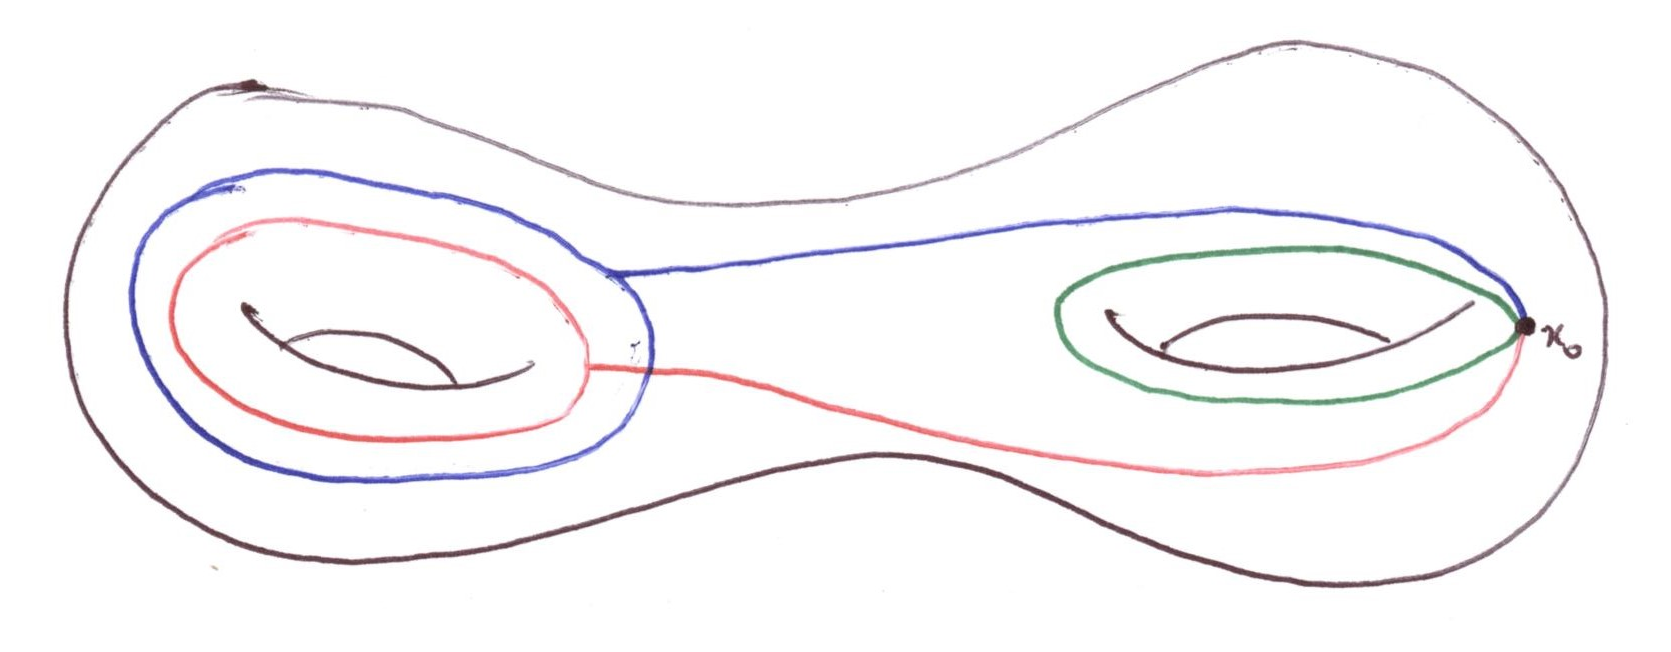
\includegraphics[scale=0.2]{conjugating_loops.png}
\end{figure}

If we have a family of pointed types over a pointed type, i.e. $X:\Type_{\pt}$ and $Y : X \to_{\pt} \Type_{\pt}$, then the type of \emph{pointed sections} is a section $s$ such that $s\ \pt = \pt$, i.e. we only specify this extra data at $\pt : X$. One canonical such section is the constant section $x \mapsto \pt : Y(x)$ and so this is itself a pointed type with the constant section as base point.

There are some lemmas about the levels of connectivity that hold for a space of pointed sections, given data about the connectivity of the base and fibers.

The action of a group $G$ on an object $a : A$ is a map $X: BG \to A$ with $X(pt) = a$. ``Clearly'' this is the same as a homomorphism $G \to \Aut_A a$. (Because a homomorphism is defined as a deloopable map and we just defined the action in terms of the delooping.)

A ``$G$-type'' is a type in the context of $BG$, i.e. a map $X : BG \to \Type$. A map of $G$-types is a function $\alpha : (z : BG) \to X(z) \to Y(z)$. This is a map for each point of $BG$. So we are calling $X$ the $G$-type, not the type $X(pt)$.

Egbert: A higher group $G$ is defined to be a pointed connected type $BG$. The underlying type of the higher group $G$ is then just the loop space of $BG$. This loop space is what $G$ really is, and its group structure comes from it being the loop space of $BG$. A $G$-type should then be a type equipped with a $G$-action. We just define it as a fibration over $BG$, so that the $G$-action comes canonically from the lifting property. So, if $X : BG \to Type$, then we have

- a type $X(*)$ at the base point
- a G-action $X(*) -> X(*)$ for every loop of $BG$

If $X$ would be a $G$-set, then the type of fixed points would be

$$\sum (x : X(*)), \prod (p : * = *), tr(p,x) = x$$

where tr is transport/lift. With a bit of abstract nonsense it follows that this is the type

$$\prod (y : BG), X(y).$$

However, if $X$ is not a $G$-set but a $G$-type, then that first type of fixed points isn't quite right, because it misses the higher coherences. It turns out that the Pi-type is the right thing :)

Greg, later. Given a type family $X$ over a base $BG$, there are two God-given constructions that together produce exactly this fixed-point story. The first is transport: given an equality in the base $x = y$, we get a \emph{function} between fibers $X(x)\to X(y)$. Since the group is the loop space at a point, the transport function is the group action. The second operation is action on paths. Given a \emph{section} $s$  of the type family and an equality $p : x = y$ in the base, we get an equality $tr(p, s(x)) = s(y)$. The narrative with this is that we can't directly compare $s(x)$ and $s(y)$ since they live in different fibers, so first we transport $s(x)$ using $p$ then compare, and we get an equality. In the special case $p : x = x$, i.e. $p \in G$, this is a fixed point for the group action. To recap, given only the group, we only get a function on the fiber (or between fibers if the equality is not a loop). But given also a section, we also get fixed points for the function. This bears further reflection.

So why do we define $X/G := \sum (y : BG), X(y)$? Quotients should have a quotient map: Here the quotient map is just the inclusion of the fiber $X(*)$. The quotient map is surjective: This follows from the fact that $BG$ is connected. The quotient map should be effective: in other words, in $X/G$ we should have

$$q(x)=q(y) \simeq \sum (g:G), gx=y$$

This identity type is a $\Sigma$-type. That's already the first hint that the quotient should be a $\Sigma$-type. And indeed a quick calculation will reveal that effectiveness indeed holds.

Greg, later: ``$gx$'' is the action of $g$, so again transport. So given $p:*=*$ we have $tr_p:X(*) \to X(*)$...

\section{The real outline}
New constructions to import into HoTT: associated bundle, gauge group, Atiyah sequence, flat connection.
\subsection{Associated bundle}
$G$-actions are type families over $BG$, and given $X\to BG$ we can pull any of these back. If we pull back $G$ (as in, the right action of $G$, as a type over $BG$), we get a principal bundle. But if we pull back another action we get the associated bundle. This puts the principal bundle and the associated bundle on the same footing -- they are all actions that we pull back.

A statement to make rigorous: if the image of $X$ is a contractible type containing pt, then the bundle is trivial.
\subsection{Gauge groupoid}
Aka $P\times_G P \to X$. The objects of the groupoid are the fibers of $P$, which of course are in 1-1 correspondence with points of $X$. The morphisms are fiber ismorphisms that are compatible with the $G$-action. This is where holonomy lives. Paths in the manifold give group actions on the fibers of $P$. The path can have separate endpoints and so we examine pairs of fibers.

This specific use of two copies of $P$ only appears when we are implicitly focused on 1-paths which have two endpoints. The right object is probably $\shape P$.

If $P:A\to BG$ is a principal bundle, and given an equality in the base $p: x =_A y$ we get by action-on-paths an equality $P(x)=_{BG}P(y)$ in $BG$, which lifts to any action we may have such as the right action $G$ or $G^{\mathrm{ad}}$.
\subsection{Atiyah sequence}
An exact/fiber sequence of groupoids. (See https://ncatlab.org/nlab/show/Atiyah+Lie+groupoid). Adjoint bundle/groupoid is what Bucholtz et all call $G^{\mathrm{ad}}$. The gauge groupoid is the middle object. And on the right we have $X\times X$, simply pairs of points. We want to replace this with $\shape X$ and so we need a map $\shape X \to X\times X$ and then pull back the diagram.
\subsection{Connection}
A connection is a splitting of the Atiyah sequence. By Schreier theory these are in correspondence with something. A splitting $X\times X \to P\times_G P $ is a trivialization? And a splitting $\shape X \to P\times_G P $ is a flat connection. That's our destination. Meanwhile there's another characterization that uses a map $X\to\flat BG$ to characterize a principal bundle \emph{with} a connection, whereas the principal bundle alone is characterized by $X\to BG$.

In Kolor-Michor-Slovak 9.8 (p. 80) they prove parametrization invariance of transport.
\subsection{Flat connection}
HoTT transport is parallel transport. But HoTT transport operates on equalities instead of paths. The shape modality converts paths into equalities. So given a manifold $X$, we form $\shape X$ and then select a bundle $\shape X \to BG$. Pulling back the right action $G$ type over $BG$, we get a principal bundle. Now any equality in the base can be lifted to an action on fibers and this can directly be interpreted as parallel transport, of a flat connection. We don't have to form the Atiyah sequence and split it, and we don't need the gauge groupoid as of yet. We already have our hands on flat connections just by using standard HoTT transport plus $\shape$.
\subsection{Connections from flat connections}
Here we will work through what Schreiber is saying in DCCT 1.2.7.1.3. Flat 2-connections with values in $\mathrm{INN}G$ model 1-connections and keep track of their curvature. (Schreiber example 1.2.127).

\subsection{Defining the path groupoid in HoTT}
A sub-goal is to define $\textbf{P}(X)$ for a type $X$ using higher inductive types. In Zulip it was suggested I follow the pattern of Licata-Finster when they defined Eilenberg-MacLane spaces. I'm reading the HoTT book chapter 6 and want to read the Cubical materials on HITs as well.

Given a type $X$ we want to set all its paths to equalities, so we will have a constructor that is a function $f:\textbf{P}(X)\to =_X$ where if $p:[0,1]\to X$ then $f(p)\in f(0)=f(1)$. Then we need higher equalities for the thin homotopies, and of course arbitrary non-thin homotopies will not be made into equalities. Perhaps thin homotopies can be described as $n$-homotopies ($n>1$) whose \emph{image} is contained in the \emph{image} of one of the two paths. This will imply that the other path's image is also a subset.

This object can then map to a higher group to create a principal bundle, and transport will be a connection. 

Can I refer to the paths in $X$ as $||\shape X||_1$?


\bibliography{connections}

\end{document}
